\documentclass[onecolumn, 12pt]{article}
  \usepackage[utf8]{inputenc}
  \usepackage{hyperref}
  \usepackage[T1]{fontenc}
  \usepackage[francais]{babel}
  \usepackage{layout}
  \usepackage{verbatim}[4]
  \usepackage{color}

  \usepackage{graphicx}
  \usepackage{caption}
  \usepackage{subcaption}

  \usepackage{titlesec}

\setcounter{secnumdepth}{4}

\title{Projet Unity}
\author{Groupe 30:\\ Seleshi Mahelet, Bachelor GSEM \\ Poggio Enzo, Master
Informatique pour sciences humaines\\ Mail:
{[}Mahelet.Seleshi,Enzo.Poggio{]}@etu.unige.ch\\ GithuB:
\url{https://github.com/EPgg92/stm} }
\date{April 2018}

\begin{document}

\maketitle
\begin{center}


\includegraphics[scale=0.5]{../Deckstop_icons/icon.png}
\end{center}

\section{Notre proposition}\label{notre-proposition}

Pour répondre aux exigences des consignes, nous souhaitons réaliser un
Rogue-Like 2D avec le moteur de jeu Unity qui sera destiné à apprendre à
additionné des chiffres (1 à 9). Nous adressons donc notre jeu à des
enfants devant apprendre à calculer rapidement.

\section{But du jeu}\label{but-du-jeu}

Notre jeu prends place dans un univers post-apocalyptique où
notre protagoniste est chassé par des Zombies. Pour aider à leur
échapper le joueur doit faire l'addition des deux tuiles spéciales sur
la grille pour trouver la bonne sortie; puis trouver le chemin vers la
bonne sortie qui évite au plus les Zombies et qui permet de ramasser le
plus de nourriture.

\section{Gameplay}\label{gameplay}

La nourriture sera notre vie. On commence une partie avec un capital de
100 de nourriture. On peut en perdre en se faisant attaquer par les
zombies (-10 ou -20) ou bien en se déplaçant (-1) ou bien encore en
prenant une mauvaise sortie (int(food/2) + 1). Le joueur pourra regagner
de la vie s'il ramasse certain pick up: des sodas (+20) ou des pommes
(+10). Certaines mauvaises sorties seront évidentes car rouge et sans
nombre dessus.

Si le protagoniste n'a plus de nourriture il meurt et c'est la fin du
jeu. La partie est perdue. Au bout d'un certain nombre de niveau (une
vingtaine) le jeux se finira. La partie est gagnée! Les niveaux seront
exprimés en nombre de jour où le protagoniste a survécu.

Ce rogue-like est un tour par tour, c'est-à-dire que tant que le joueur
n'effectue pas votre action les ennemies n'effectuent pas la leur. Le
joueur à deux types d'action: se déplacer dans une direction cardinal et
casser un mur qui gène le passage.

\section{Nos règles
d'adaptivité}\label{nos-ruxe8gles-dadaptivituxe9}

La difficulté sera progressive et constante. Elle se base uniquement sur
le nombre d'ennemies qui vont spawn au début de chaque salle.
\begin{center}
\begin{figure}
   \caption{\label{difficulty} Courbe d'augmentation du nombre d'ennemies}
   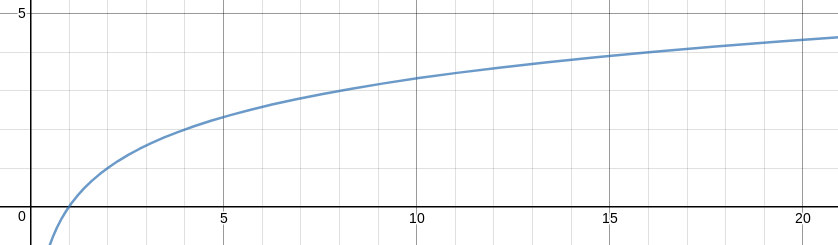
\includegraphics[scale=0.45]{../img/difficulty.png}
\end{figure}
\end{center}


Ainsi on aura 1 ennemie à partir du niveau 2, puis 2 à partir du niveau
4, puis 3 à partir du niveau 8, et finalement 4 à partir du niveau 16.

Si il nous reste du temps nous ferons un adaptation de la difficulté
dans le calcul aussi. C'est à dire plus on va dans des niveaux élevés
plus les chiffres seront grands. Et plus les mauvaises sorties auront des
résultats proches de la bonne sortie.

\section{Structure du jeu
prévue}\label{structure-du-jeu-pruxe9vue}

\subsection{Scène}\label{scuxe8ne}

Nous n'aurons qu'une scène dans notre jeu où le plateau de déplacement
ne sera que de 8 par 8 (avec les bordures infranchissables 10 par 10). À
chaque nouvelle partie et nouveau niveau le plateau sera totalement
régénéré aléatoirement.

\subsection{Gameobjects}\label{gameobjects}

Tous nos gameobjects seront sauvés en temps que prefabs:

\begin{itemize}

\item
  \textbf{Player} : prefab du sprite du protagoniste contrôlé par le
  joueur.
\item
  \textbf{Enemy} : 2 prefabs pour 2 sprites d'ennemies différents.
\item
  \textbf{Exit} : 24 prefabs de sortie; une mentionnant juste ``Exit''
  pour la fin du jeu; 17 sorties numérotés de 2 à 18 pour les calculs; 6
  sorties en rouge piège.
\item
  \textbf{Floor} : 8 prefabs pour 8 sprites de sols différents.
\item
  \textbf{SpcialFloor} : 9 prefabs pour 9 sprites de sols numérotés de 1
  à 9.
\item
  \textbf{Food} : prefabs du pick up avec le sprite de pommes.
\item
  \textbf{Soda} :prefabs du pick up avec le sprite de sodas.
\item
  \textbf{Wall} : 8 prefabs pour 8 sprites de murs différents.
\item
  \textbf{OuterWall} : 3 prefabs pour 3 sprites de murs extérieurs
  différents.
\end{itemize}

\subsection{Scripts}\label{scripts}

\begin{itemize}

\item
  \textbf{GameManager}: Permet d'initialiser les différentes instances
  du jeu.
\item
  \textbf{BoardManager}: Permet de créer le plateaux de déplacement.
\item
  \textbf{SoundManager}: Permet d'exécuter les interactions sonores du
  jeu.
\item
  \textbf{Loader}: Empêche de créer une nouvelle instance du jeux si existante, en crée une si nécessaire.
\item
  \textbf{MovingObject}: Permet de définir comment vont bouger nos Units
  (Player et Enemy).
\item
  \textbf{Enemy}: Définit les différentes actions des ennemies.
\item
  \textbf{Player}: Définit les différentes actions du joueur.
\item
  \textbf{Wall}: Permet de gérer la destruction d'un mur par le joueur.
\end{itemize}

\section{Ressources utilisées}\label{ressources-utilisuxe9s}

Nous allons utiliser un assortiment d'assets et de tutoriels proposés
sur l'Asset Store de unity:

\begin{itemize}

\item
  \href{https://unity3d.com/fr/learn/tutorials/s/2d-roguelike-tutorial}{2D
  Roguelike tutorial}
\item
  \href{https://www.youtube.com/watch?v=Fdcnt2-Jf4w\&list=PLX2vGYjWbI0SKsNH5Rkpxvxr1dPE0Lw8F}{Tutoriels
  Vidéos}
\end{itemize}
\end{document}
